\chapter{Semafori}
\section{Problemi di mutua esclusione e di sincronizzazione}
Gli utenti del nostro sistema possono creare processi e far eseguire funzioni scelte da loro. Questo utente può definire tanti processi; inoltre, questi processi hanno accesso a una memoria comune (le sezioni \emph{text}, \emph{data} e \emph{bss}).
\paragraph{Altri problemi} Questi processi possono mescolarsi fra loro e possono agire su strutture dati condivise. Come può l'utente garantire che tutto funzioni correttamente? Il problema è simile a quello del modulo sistema (ricordare l'esempio delle liste inconsistenti): li abbiamo risolto con l'atomicità (interruzioni esterne disabilitate, evitiamo eccezioni e chiamate ricorsive di primitive del sistema). Il fatto è che non possiamo permettere all'utente di disattivare le interruzioni, potrebbe non attivarle più e impedirci di riprendere il controllo. Classifichiamo le questioni.
\begin{itemize}
	\item \textbf{Problemi di mutua esclusione}.
	
	L'utente deve fare una o più azioni su una stessa struttura dati, ma non vuole che queste azioni vengano fatte contemporaneamente (cioè non vuole che si mescolino con altre azioni). Si definiscono più processi che possono lavorare sulla stessa lista: queste devono essere mutuamente esclusive, se una cosa è in esecuzione allora l'altra non deve essere in esecuzione.
	
	\item \textbf{Problemi di sincronizzazione}.
	
	L'utente vuole che una certa azioni si verifichi sempre prima di un'altra. In presenza di un sistema multiprocesso può essere molto complicato (se non impossibile) capire a priori l'ordine in cui i processi saranno eseguiti. Esempio: definizione della struttura dati e lettura della struttura dati, la seconda operazione non ha senso finchè la prima operazione non viene conclusa (\emph{produttore} vs \emph{consumatore}).
\end{itemize}
Non ci addentriamo molto in queste questioni, vedremo solo ciò che ci serve. Attenzione a non confondere le due cose:
\begin{itemize}
	\item nel problema di mutua esclusione non ci interessa l'ordine delle operazioni, ci basta solo non avere il mescolamento delle stesse;
	\item nel problema di sincronizzazione la questione è proprio l'ordinamento.
\end{itemize}

\section{Soluzione ai problemi introdotti: le primitive semaforiche} 
Il sistemista non può risolvere a priori le questioni introdotte, visto che solo l'utente sa cosa vuole fare. Quello che faremo è fornire all'utente le cosiddette \textbf{primitive semaforiche}.
\paragraph{Metafora}  Diamo all'utente la possibilità di definire delle scatole di gettoni, cioè scatole che possono contenere dei gettoni. Posso fare solo due operazioni: inserire un gettone, prendere un gettone. La particolarità sta nella seconda operazione: la scatole è opaca, non sappiamo quanti gettoni ci sono dentro, se nel provare a prendere il getto non trovo nulla allora l'utente si congela e non fa altro, in attesa che qualcun altro aggiunga un gettone.

%\paragraph{Primitive che ci servono} 
%\begin{itemize}
%	\item Primitive per la creazione della scatole di gettoni, indicando il numero di gettoni iniziali (anche zero).
%	\item Primitiva per l'aggiunta di un gettone nella scatola.
%	\item Primitiva per prendere un gettone dalla scatola
%\end{itemize}
%Di per sè non risolvono il problema: l'utente deve imporsi delle regole.


\subsection{Risoluzione del problema della mutua esclusione}
Prendiamo una situazione reale per capire meglio.
\begin{itemize}
	\item Durante l'esame in presenza una sola persona alla volta va in bagno. L'ordine degli studenti non mi interessa, voglio solo evitare che due studenti vadano in bagno insieme. 
	\item Risolviamo la cosa con una scatola avente un solo gettone: chi deve andare in bagno prende il gettone, e lo rimette dopo essere tornato. 
	
	\item \textbf{Problemi di persone che prendono in contemporanea il gettone?} 
	
	No, risolto a priori grazie all'atomicità delle primitive di sistema. 
\end{itemize}
\paragraph{Soluzione cooperativa} La soluzione appena descritta, coi gettoni, è detta \emph{soluzione cooperativa}. Questo perchè ci si aspetta che chi ha preso il gettone lo restituisca. Se ciò non avviene tutti gli altri non possono muoversi.




\subsection{Risoluzione del problema della sincronizzazione}
\paragraph{Cosa vogliamo fare} Supponiamo di avere un'azione $A$ e un'azione $B$. L'ordine nel complesso non ci interessa, ci basta che $A$ venga eseguita prima di $B$, SEMPRE!
\paragraph{Esempio con un buffer}
Prendiamo come esempio un buffer: abbiamo un produttore $P1$, che inserisce un contenuto, e $P2$, consumatore, che lo deve utilizzare.  Se $P2$ arriva prima si troverà ad elaborare dati casuali, e noi non vogliamo che ciò avvenga.\begin{center}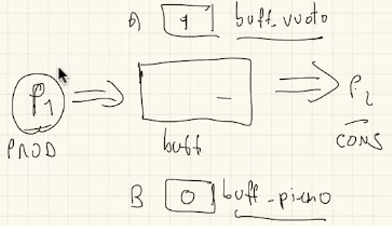
\includegraphics[scale=.8]{img/192.PNG}\end{center}
\begin{itemize}
	\item Stavolta non ho una sola scatola, ma due! 
	\item \textbf{Cosa c'è inizialmente in queste scatole?}  
	
	Una ha un gettone e una è vuota.
	
	\item\textbf{Come si usano queste scatole?}
	
	Possiamo immaginare le due scatole come delle variabili logiche, che hanno come valore $0$ o $1$. Chiamiamo la scatola $A$ \emph{buff$\_$vuoto} e la $B$ \emph{buff$\_$pieno}.
	\begin{itemize}
		\item La scatola $A$ indica se il buffer è vuoto, cioè se $P2$ ha già letto o meno il contenuto presente.
		\item La scatola $B$ indica se il buffer è pieno, cioè se $P2$ ha del contenuto nuovo da leggere.
	\end{itemize}
	Il produttore $P1$ può procedere solo se il buffer è vuoto, quindi con $A=1$ e $B=0$: segue che all'inizio $A$ avrà un gettone e $B$ non avrà gettoni. Il consumatore attende che il buffer si riempa, e agisce solo con $A=0$ e $B=1$. L'idea base è che $P1$ e $P2$, quando svolgono $A$ e $B$ (rispettivamente) levano il gettone dove è presente e lo spostano dove non c'è niente. Quindi
	\begin{itemize}
		\item Il consumatore fa le seguenti cose
		{
			\small \begin{verbatim}
				PRENDERE(buff_pieno) ---> WAIT(buff_pieno)
				CONSUMARE
				AGGIUNGERE(buff_vuoto) ---> SIGNAL(buff_vuoto)
		\end{verbatim}
	}
		\item Il produttore fa le seguenti cose
		{
			\small \begin{verbatim}
				PRENDERE(buff_vuoto) ---> WAIT(buff_vuoto)
				PRODURRE
				AGGIUNGERE(buff_pieno) ---> SIGNAL(buff_pieno)
		\end{verbatim}
	}
	\end{itemize}
	\item Si osservi che risolvendo questo problema abbiamo affrontato pure la mutua esclusione. In generale i due problemi vanno affrontati singolarmente.
\end{itemize}